% !TEX root = notes.tex
\section{Modeling}\label{sec:modeling}
In this section, we investigate how state-of-the-art KR systems without support for higher order logic, such as IDP and ASP, can model the graph mining problem 
%and its higher order features
using encoding techniques.
We identify the desirable properties that from a KR perspective should hold for a good model of the graph mining problem and we evaluate how a modeling in ProB, as a KR language with support for higher order sets, satisfies these properties.
%We conclude with a comparison of the performance of the three approaches. 

\subsection{IDP}
%We assume some familiarity with the IDP system.
%\cite{WarrenBook/DeCatBBD16} provide an extensive introduction for those who are not sufficiently familiar with the IDP system. %can be found in~\cite{}.
\subsubsection{Existential Second Order}
The IDP language allows problem specifications written in \emph{first order} (FO) theories $T$, extended with types, arithmetic, aggregates, and inductive definitions.
\textbf{Listing}~\ref{lst:vocabularyExample} shows an example.
\todo{scoped or quantified}
The symbols in these theories can be quantified locally, or quantified implicitly in the vocabulary $V$.
Symbols quantified locally can only be propositional, whereas the vocabulary can contain first order symbols such as functions or predicates, making it a \emph{second order object}.

In the graph mining problem, we are looking for an interpretation $I$ of the symbols in vocabulary $V$ such that $I$ satisfies T, called a model.
This corresponds to existential quantification of all (including FO) symbols in $V$.
\textbf{Listing}~\ref{lst:vocabularyExample} shows an example of how IDP extends a given interpretation \lstinline{S} into a model \lstinline{Result}.
Due to the existential quantification of symbols in $V$, and the lack of locally quantifiable FO symbols, IDP is limited to model expansion for \emph{existential second order} problems, which does not include graph mining.
We now expand on the underlying shortcomings, and how to sidestep them.
%The IDP language can express problems that consist of a set of symbols, called the vocabulary $V$, and a theory, called $T$, that uses symbols from this vocabulary.
%The symbols in the vocabulary can be propositions, but they can also represent predicates and functions.
%These last two types of symbols make the vocabulary, in general, a \emph{second order} object: it is an object that itself \emph{contains} not only propositional symbols, but also first order symbols.
%For example, vocabulary $V$ in \textbf{Listing} \ref{lst:vocabularyExample} is a second order vocabulary as it contains the first order symbol \lstinline{Edge/2}.
%
%The theory $T$ is restricted to a \emph{first order} theory, extended with types, arithmetic, aggregates, and inductive definitions.
%An example of such a theory is given in \textbf{Listing} \ref{lst:vocabularyExample}.
%It contains an inductive definition for \lstinline{Path/2}, and one constraint.
%
%Our inference of choice in the graph mining problem is model expansion; we search for an interpretation $I$ of symbols in the vocabulary $V$, called a \emph{model}, such that this interpretation $I$ satisfies the theory $T$.
%This corresponds to the implicit \emph{existential quantification} of all symbols in the vocabulary, both the propositional as well as the first order symbols.
%In the example of \textbf{Listing}~\ref{lst:vocabularyExample}, we expand the given interpretation $S$ to the model $Result$ with 3 edges: One from the first node to itself, one from the first node to the second, and one from the second to the third.
%Path contains all corresponding paths between these three nodes.
%
%In conclusion, we say the IDP language can express model expansion for \emph{Existential Second Order} problems.
%This level of expressiveness is not sufficient for general graph mining problems.
%We will discuss the several issues in the remainder of this section.


\begin{lstlisting}[mathescape,style=model,caption={IDP example using inductive definitions}, label=lst:vocabularyExample]
vocabulary V{
    type Node, 
    Edge(Node, Node), Path(Node, Node)
}
theory T : V {
    $\forall$n[Node] : $\exists$n2[Node] : Edge(n,n2) $\lor$ Edge(n2,n).
    {
        Path(x,y) $\leftarrow$ Edge(x,y).
        Path(x,y) $\leftarrow \exists$z[Node] : Path(x,z) $\land$ Path(z,y).
        Path(x,y) $\leftarrow$ Path(y,z).
    }
}
structure S : V{ Node = {1;2;3} }
structure Result : V{
    Node = {1; 2; 3}, Edge = {1,1; 1,2; 2,3}
    Path = {1,1; 1,2; 1,3; 2,1; 2,2; 2,3; 3,1; 3,2; 3,3 }
}
\end{lstlisting}


%problems in which there is an existentially quantified, generally second order, vocabulary of symbols and a first order theory with symbols from that vocabulary.
\paragraph{Issue 1}
First, we must represent the sets of example graphs, as specified in \textbf{Def.}~\ref{def:gm2}.
One possible way is shown \textbf{Listing}~\ref{lst:HOPred}, which uses a higher order predicate \lstinline{PositiveGraph/3} with the node predicate, edge predicate and labeling function as arguments. 
The first graph consists of nodes 1 (labeled a), 2 (labeled b) and is fully connected.
%This definition uses a higher order predicate \lstinline{GraphInst/3} (See \textbf{Listing}~\ref{lst:HOPred}) with the edge predicate as first argument and the labeling function as second argument. For the first graph, \lstinline|{1,2; 2,1}| and \lstinline[mathescape]|{1$\mapsto$ a; 2$\mapsto$ b}| respectively.
This highly locally coherent representation preserves a graph as an independent tuple of predicates and functions.
However, our vocabulary $V$ cannot contain such a second-order symbol.
%It represents a single graph as a tuple of predicates and functions, which is a highly locally coherent representation, preserving the independence of graph characteristics.
%, visualized in \textbf{Fig.}~\ref{fig:LocalCoherence} as the solid shape.
%It is clear that this representation is highly locally coherent, and preserves the independence of graph characteristics.
%However, as we are restricted to \emph{Existential} Second Order, we cannot express this higher order predicate in IDP.

One possible solution is to replicate for each graph the different characteristic predicates and functions, as shown in \textbf{Listing}~\ref{lst:multiglobal}.
%Because now there is no relation between the different edge predicates and label functions, it is necessary to formulate our theory in terms of these different predicates and functions.
Encoding a property such as ``In every graph, all nodes have at least two outgoing edges'' must be stated for every graph and its edge predicate explicitly, as no relation exists between the different edge predicates and label functions:
%duplicate in our theory the constraints and properties (i.e. homomorphism) about these example graphs and their relations as well: we cannot generalize over the names of these edge relations and labeling functions.

%\vspace{-0.5em}
\begin{minipage}{\linewidth}
\begin{center}
\begin{lstlisting}[style=small,mathescape]
$\forall$ n[Node] : $\exists$ n1,n2[Node] : E1(n, n1) $\land$ E1(n,n2) $\land$ n1 $\neq$ n2.
$\forall$ n[Node] : $\exists$ n1,n2[Node] : E2(n, n1) $\land$ E2(n,n2) $\land$ n1 $\neq$ n2.
\end{lstlisting}
\end{center}
\end{minipage}
\noindent It is clear that this solution is undesirable due to the way it scales 
%and the theory modifications needed
with growing problem instances: it prohibits the abstraction (generalization) of knowledge in the theory.

%It retains the local coherence and independence of graph characteristics when it comes to data representation, but prohibits the abstraction (generalization) of knowledge in the theory.
% about these properties, as evidenced by our obligation to duplicate the theory for each graph.
\begin{minipage}{\linewidth}
\begin{center}
\begin{minipage}{0.80\linewidth}
  \begin{lstlisting}[style=small,mathescape,caption=Higher order predicate modeling the set $\graphset{G}_{+}$ of \textbf{Def.}~\ref{def:gm2}.,label=lst:HOPred]
PositiveGraph({1,2}, {1,2; 2,1},{1$\mapsto$a; 2$\mapsto$b}).
PositiveGraph({1,2,3}, {1,3; 2,1},{1$\mapsto$c; 2$\mapsto$b; 3$\mapsto$a}).
\end{lstlisting}
\end{minipage}
\end{center}
\vspace{-2em}

\begin{minipage}[t]{0.45\linewidth}
\begin{lstlisting}[style=small,mathescape,caption=Multiple individual global relations,label=lst:multiglobal]
E1(1,2). lb1(1)=a.
E1(2,1). lb1(2)=b.
E2(1,3). lb2(1)=c.
E2(2,1). lb2(2)=b.
         lb2(3)=a.
\end{lstlisting}
\end{minipage}
\begin{minipage}[t]{0.1\linewidth}
 ~
\end{minipage}
\begin{minipage}[t]{0.45\linewidth}
\begin{lstlisting}[style=small,mathescape,caption=Disjoint union using indexed global relations,label=lst:indexedglobal]
E(g1,1,2). lb(g1,1)=a.
E(g1,2,1). lb(g1,2)=b.
E(g2,1,3). lb(g2,1)=c.
E(g2,2,1). lb(g2,2)=b.
           lb(g2,3)=a.
\end{lstlisting}
\end{minipage}
\end{minipage}

A more workable solution is to represent each characteristic property, such as the edge relation, by a single global relation for all graphs, as shown in \textbf{Listing}~\ref{lst:indexedglobal}.
% and by the dotted shape in \textbf{Fig.}~\ref{fig:LocalCoherence}.
This relation behaves the way it should for a specific graph instance based on an additional argument serving as an identifier for the graph of interest.
%This gives rise to a set $G$ of \emph{graph identifiers}, one for each example graph.
This global edge relation now corresponds to the \emph{disjoint} or \emph{tagged union} of the graphs' edge relations, with tags drawn from a set \lstinline{G} of graph identifiers.
It is clear that this representation forces us to give up the local coherence of graph characteristics that was present in \textbf{Def.}~\ref{def:gm2}.
%Nu kunnen we kijken wat deze truuk doet met onze mogelijkheid om de abstraction van de theory uit te drukken. Normaal mwillen we dit zo schrijven. Hoewel we nu de generalisatie kunnen uitdrukken, verplicht de restrictie tot existentieel s..o ons om de homomorphic mapping functies te tot een globale property te promoveren, hoewel we feitelijk niet geinteresseerd zijn in de concrete mappings. om om te gaan met de afhankelijkheid van deze functies op de spec. vb grafen moeten we... die nu erg lijkt op skolemisation. theory
%
%Using this trick however, does not influence our ability to 
However, generalizing over the different graphs, we can now encode the property stated above as:
\begin{center}
\begin{minipage}{1.02\linewidth}
\vspace{-2em}
\begin{lstlisting}[style=small,mathescape]
$\forall$ gid[G] : $\forall$ n[Node] : $\exists$ n1,n2[Node] : E(gid, n, n1) $\land$ E(gid, n,n2) $\land$ n1 $\neq$ n2.
\end{lstlisting}
\end{minipage}
\vspace{-3em}
\end{center}
%\vspace{-1em}
%\begin{figure}[h]
%\centering
%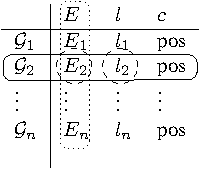
\includegraphics{CoherenceTable-crop.pdf}
%\caption{Local coherence\label{fig:LocalCoherence}}
%\vspace{-2em}
%\end{figure}

\paragraph{Issue 2}
%Having solved\matthias{circumvented?} our first issue, 
The homomorphic property can be expressed using a count aggregate, as shown in \textbf{Listing}~\ref{lst:QuantifyOutsideVocabulary}.
First we quantify over all example graphs $g$, or per \textit{Issue 1}, their identifiers, and subsequently express that there must exist a function $f$ that represents a homomorphism from our pattern graph $\graph{P}$ to $g$.
%Next, we would like to express the homomorphic property.
%This can be done using a count aggregate, as shown in Listing~\ref{lst:QuantifyOutsideVocabulary}.
%First we express the set of all example graphs to whom there exists a homomorphism from our pattern $\graph{P}$.
% generate the set of all example graphs to whom we can find a homomorphism from our pattern.
%We do this by quantifying over all example graphs g or, per \textbf{issue 1}, their identifiers, and subsequently 
%expressing the condition under which they are part of this set: i.e. that there must exist a function f that represents a homomorphism from our pattern graph $\graph{p}$ to $g$.
%In principle, we could then proceed by counting the number of elements in this set.
\begin{center}
\begin{minipage}{0.75\linewidth}
\vspace{-1em}
\begin{lstlisting}[style=small,mathescape, caption=Quantifying over functions outside the vocabulary, label=lst:QuantifyOutsideVocabulary]
#{g $\mid$ g $\in$ $\graphset{G}_{+}$ $\land \exists$ f : f is a homomorphism from $\graph{P}$ to g} $\geq$ N$_{+}$
\end{lstlisting}
\vspace{-0.75em}
\end{minipage}
\end{center}
However, IDP forbids us from locally quantifying over first order symbols such as the function  \lstinline{f} from \textbf{Listing}~\ref{lst:QuantifyOutsideVocabulary}.
%However, IDP restricts us to Existential Second Order, which forbids us from quantifying over first order entities such as the function $f$ from \textbf{Listing}~\ref{lst:QuantifyOutsideVocabulary} outside of the vocabulary.
%However, working in IDP, the restriction to ESO forbids us to quantify over first order entities such as the functions f from \textbf{Listing}~\ref{lst:QuantifyOutsideVocabulary} outside of the vocabulary.
We must promote the homomorphic functions to a symbol in the vocabulary, even though we are only interested in the existence of a mapping, not its identity.
Reusing the disjoint union technique proposed above, we can prevent having to introduce a homomorphic function for each example graph separately.
%We prevent the same explosion of mapping functions as with the graph characteristics in \textit{Issue 1}, by reusing the disjoint union technique proposed above. 
%Note that in this case, the disjoint union technique greatly resembles Skolemization. 
Note, we introduce a function \verb|f| representing all homomorphisms, and explicate its dependency on a specific example graph using an additional argument \lstinline{gId}.
%As it is impossible
%We introduce a general function \verb|f| that represents the homomorphisms, and make its dependency on a specific goal graph explicit using an additional argument:
In Second Order Logic, this dependency would follow directly from the syntactic order of the quantifications.

\begin{center}
\begin{minipage}{0.80\linewidth}
\vspace{-1em}
\begin{lstlisting}[style=small,mathescape, caption=Globalized existential functions, label=lst:GlobalizeExistentialQuantifications]
#{gId $\mid$ gId $\in$ $\graphset{G}_{+}$ : f(gId) is a homomorphism from $\graph{P}$ to gId} $\geq$ N$_{+}$
\end{lstlisting}
\vspace{-1em}
\end{minipage}
\end{center}
While all example graphs have an \lstinline{edge}, \lstinline{label}, \ldots relation, not all example graphs have a homomorphic function.
Therefore, \lstinline{f} is not defined for graph identifiers that correspond to such graphs, meaning \lstinline{f} has become a partial function.
%We can now use this \verb|f| anywhere we would use the regular homomorphic function for a specific graph by fixing the chosen example graph.
%We denote by $f(g)$ the function $f$ partially applied on argument $g$.
%However, for some example graphs $\graph{G}$, there will not exist a homomorphic function from our pattern $\graph{P}$ to $\graph{G}$, i.e. for these graphs $\graph{G}$, no valid function $f$ exists.
%Because the disjoint union technique introduces a single function $f$ which is the union of all these smaller functions, function $f$ becomes partial: it is not defined for tuples where the first the argument is an identifier for a graph $\graph{G}$ for which no homomorphic function exists.


%\todo{Of course, other (even uglier) schemes exist to encode this. Should we mention this?}


\paragraph{Issue 3} 
%The problem of deciding whether a homomorphism from one graph to another exists is \NP-complete.
%As a result, deciding that no homomorphism from one graph to another exists, which forms the basis for the negative homomorphic property, is \coNP.
Deciding that no homomorphism from one graph to another exists, as necessary for the negative homomorphic property, is \coNP.
As an \NP\ (or $\Sigma^{p}_{1}$) solver, IDP cannot solve this problem directly.
One might be tempted to simply specify the negative homomorphic property simply as: 
\lstinline[mathescape]|#{g $\mid$ g $\in$ $\graphset{G}_{-}$: f(g) is a homomorphism from $\graph{P}$ to g}$\leq$ N$_{-}$|.
%Consider, for example the template, pattern candidate and positive and negative example graphs from \textbf{Fig.}~\ref{fig:ex2}, and assume all nodes have the same label.
%With parameters $N_{+}=1$ and $N_{-}=0$, this pattern candidate is clearly an invalid pattern: It is homomorphic with both the positive and the negative example.
%When one would use the most straightforward encoding of the negative homomorphic property, one would reuse our result from \textbf{Issue 2}, and state:
%The straightforward encoding of the negative homomorphic property reuses the result from \textit{Issue 2}:
%\begin{center}
%\begin{minipage}{0.65\linewidth}
%\vspace{-1em}
%\vspace{-1em}
%\begin{lstlisting}[style=small,mathescape]
%#{$g \mid g \in G$ : $f(g)$ is a homomorphism from $\graph{P}$ to $g$}$\leq$ N$_{-}$
%\end{lstlisting}
%\vspace{-1em}
%\end{minipage}
%\end{center}

However, the IDP solver has no obligation to maximize the number of homomorphisms it finds for \lstinline{f}, only to satisfy the constraints.
Thus, it can choose \lstinline{f} such that it does not represent a homomorphism for a graph \lstinline[mathescape]{g $\in$ $\graphset{G}_{-}$}.
As our constraints are satisfied, we are led to believe that our pattern candidate is a valid pattern.
%Thus, even if there is a negative example $\graph{G}_{-}$ for which a homomorphism exists, the solver can choose $f$ such that $f$ does not represent a homomorphism for this graph $\graph{G}_{-}$.

%But now, our solver must choose a single global function $f$ which satisfies the constraints.
%It has no obligation to maximize the number of homomorphisms in $f$, only to satisfy the constraints.
%Thus, even if there is a negative example $\graph{G}_{-}$ for which a homomorphism exists, the solver can choose $f$ such that $f$ does not represent a homomorphism for this graph $\graph{G}_{-}$.
%An example of such a model is shown in Listing~\ref{lst:invalidf}: this function $f$ maps the pattern candidate's nodes $1, 2, 3$ to $a, b, c$ for the positive example, i.e. f is a homomorphism, but maps $1, 2, 3$ to $d, e,$ and $g$ for the negative example.
%Now, even though it is possible to find a homomorphism between the pattern candidate and the negative example (by mapping $3$ to $f$ instead)
%As our constraints are satisfied, we are led to believe that our pattern candidate is a valid pattern.

\citep{conf/fsttcs/Immerman98} has shown that this is inherently linked to IDPs limit to Existential Second Order.
Indeed, checking that our pattern \graph{P} is homomorphic with no more than $N_{-}$ negative graphs is equivalent with checking that enough negative examples \lstinline{G} exist for which  no homomorphism exists (\textbf{Listing}~\ref{lst:universalquant}). This clearly leads to a universal quantification over a function variable, which IDP cannot express.
%Indeed, in order to check that our pattern \graph{P} is homomorphic with no more than $N_{-}$ negative graphs, we have to check that there are enough negative graphs for which no homomorphism exists, for example using a count aggregate as in \textbf{Listing}~\ref{lst:universalquant}.
%By asserting a property for all candidate homomorphic functions $f$ of a certain graph $g$, the negative homomorphic constraint leads to universal quantification over a function variable.

\vspace{-1.25em}
\begin{center}
\begin{minipage}{0.75\linewidth}
\begin{lstlisting}[style=small,mathescape, caption=Quantifying over functions outside the vocabulary, label=lst:universalquant]
#{$g \mid g \in \graphset{G}_{-} \land \forall$ $f$ : $f$ is $\mathbf{not}$ a homomorphism from $\graph{P}$ to $g$}
\end{lstlisting}
\end{minipage}
\end{center}
\vspace{-0.5em}

A way to work around this is by encoding the dual (i.e. negated) problem, and conclude that the problem is satisfied if and only if no model exists for the dual problem.
%A way to solve a \coNP\ problem such as the negative homomorphism constraint using an \NP\ solver is by encoding the dual (i.e. negated) problem, and conclude that the problem is satisfied if no model exists for the dual problem.
This can be checked using an \NP\ solver.
However, this technique can only be implemented in IDP by writing two theories: 
\begin{compactitem}
\item one (positive) theory $\theory^{+}$ (see Appendix \ref{app:Code}), which expresses the positive homomorphic property and generates pattern candidates, and
\item one negative theory $\theory^{-}$, which expresses the (dual of) negative homomorphic property and rejects pattern candidates that do not satisfy this constraint.
\end{compactitem}
In IDP, one must provide procedural code that ties these two theories and their inferences together, allowing pattern candidates to be communicated between them.

It is not known whether the problem of graph isomorphism is polynomial time solvable,
however it is sure to be no more complex than NP.
Conversely, the isomorphism restriction when looking for multiple patterns is also no more complex than \coNP.
Therefore, we can use the same technique, giving rise to another theory $\theory^{iso}$.
Note that it is possible to combine the negative theories $\theory^{-}$ and $\theory^{iso}$ into a single negative theory.


%Much in the same way, limiting ourselves to existential second order prohibits us from expressing the negative homomorphic property (the pattern is homomorphic with no more than $N_{-}$ negative examples) in the same model.
%In fact, the negative homomorphic constraint asserts a property for all candidate homomorphic functions, which would lead to \emph{universal} quantification.
%Therefore, our only recourse is to encode its dual positive constraint and require it to fail when queried.

%Take, for example, the template, pattern candidate and positive and negative example graphs from \textbf{Fig.}~\ref{fig:ex2}.
%Assume all nodes have the same label.
%With parameters $N_{+}=1$ and $N_{-}=0$, this pattern candidate is clearly an invalid pattern: It is homomorphic with both the positive and the negative example.
%Suppose we express the negative homomorphic property directly, changing only the comparison operator used on the count aggregate from $\geq$ to $\leq$.
%Because we now look for one general (Skolemized) homomorphic function, we can choose a single global function which represents a homomorphism with the positive example graph, but not with the negative example graph.
%An example of such a solution is shown in Listing~\ref{lst:invalidf}.

%If we want to prevent these invalid models, we must encode the dual positive constraint, and require it to fail. 
%However, to do this in IDP, we need another theory and provide procedural (lua) code that ties these theories and their inferences together. 
%It must pass models from the theory that asserts the positive property to the theory that checks the negative property. This procedural code is clearly not declarative.
%In much the same way, IDP cannot express the isomorphism restriction when looking for multiple patterns: if needed, this restriction is transformed into a dual positive restriction (there \emph{must} be an isomorphism) and is required to fail as well. These two theories expressing the dual of the negative homomorphism property and that of the isomorphism restriction can safely be merged.

%%\begin{figure}
%%  \centering
%%  \begin{subfigure}[b]{0.15\textwidth}
%%    \centering
%%    \begin{tikzpicture}[scale=.35]
%%      \node[vertex] (a) at (1,1) {};
%%      \node[vertex] (b) at (2,1) {};
%%      \node[vertex] (c) at (2.7,2) {};
%%      \node[vertex] (d) at (2,3) {};
%%      \node[vertex] (e) at (1,3) {};
%%      \node[vertex] (f) at (0.3,2) {};
%%      
%%      \draw (1,1) -- (2,1) -- (2.7,2) -- (2,3) -- (1,3) -- (0.3,2) -- (1,1);
%%      \draw (1,1) -- (2,3);
%%      \draw (2.7,2) -- (0.3,2);
%%      \draw (1,3) -- (2,1);
%%    \end{tikzpicture}
%%    \caption{Template}
%%  \end{subfigure}
%%  ~
%%  \begin{subfigure}[b]{0.22\textwidth}
%%    \centering
%%    \begin{tikzpicture}[scale=.35]
%%      \node[vertex] (a) at (1,1) {};
%%      \node[vertex] (b) at (2,1) {};
%%      \node[vertex] (c) at (2.7,2) {};
%%      \node[vertex] (d) at (2,3) {};
%%      \node[vertex] (e) at (1,3) {};
%%      \node[vertex] (f) at (0.3,2) {};
%%      
%%      \node[circle] at (1,0.7) {a};
%%      \node[circle] at (2,0.7) {b};
%%      \node[circle] at (3,2) {c};
%%      \node[circle] at (1.6,3.8) {g1};
%%      \draw (1,1) -- (2,1) -- (2.7,2) -- (2,3) -- (1,3) -- (0.3,2) -- cycle;
%%      \draw (1,1) -- (2,3);
%%      \draw (2.7,2) -- (0.3,2);
%%    \end{tikzpicture}
%%    \caption{Positive Example}
%%  \end{subfigure}
%%  ~
%%  \begin{subfigure}[b]{0.23\textwidth}
%%    \centering
%%    \begin{tikzpicture}[scale=.35]
%%      \node[vertex] at (0,0) {};
%%      \node[vertex] at (1,1) {};
%%      \node[vertex] at (2,0) {};
%%      \node[vertex] at (3,1) {};
%%    
%%      \node[] at (0,-0.2) {d};
%%      \node[] at (1,1.2) {e};
%%      \node[] at (2,-0.2) {f};
%%      \node[] at (3,1.2) {g};
%%      \node[] at (1.6, 2.8) {g2};
%%      \coordinate (1) at (0,0);
%%      \coordinate (2) at (1,1);
%%      \coordinate (3) at (2,0);
%%      \coordinate (4) at (3,1);
%%      \draw (1) -- (2) -- (3) -- (4);
%%    \end{tikzpicture}
%%    \caption{Negative Example  \label{fig:ex2-neg}}
%%  \end{subfigure}
%%  ~
%%  \begin{subfigure}[b]{0.22\textwidth}
%%      \centering
%%      \begin{tikzpicture}[scale=.35]
%%        \node[vertex] at (1,2) {};
%%        \node[vertex] at (2,3) {};
%%        \node[vertex] at (3,3) {};
%%        
%%        \node[circle] at (0.9,2) {1};
%%        \node[circle] at (2,3.3) {2};
%%        \node[circle] at (3.15,3.3) {3};
%%        \draw (1,2) -- (2,3) -- (3,3);
%%      \end{tikzpicture}
%%      \caption{Pattern Candidate \label{fig:ex2-cand}}
%%  \end{subfigure}
%%  \caption{Example 2\label{fig:ex2}}
%%\end{figure}
%%
%\begin{minipage}{\linewidth}
%%    \begin{minipage}{0.5\linewidth}
%%    \begin{lstlisting}[mathescape,caption={A possible assignment for f s.t. it represents no homomorphism from Fig.~\ref{fig:ex2-cand} to Fig.~\ref{fig:ex2-neg}}, label=lst:invalidf]
%%f={
%%    g1,1$\mapsto$a; g1,2$\mapsto$b; g1,3$\mapsto$c;
%%    g2,1$\mapsto$d; g2,2$\mapsto$e; g2,3$\mapsto$g
%%}
%%    \end{lstlisting}
%%    \end{minipage}
%    \begin{minipage}{0.5\linewidth}
%    \centering
%    \begin{tikzpicture}[scale=0.7]
%       \node[vertex] at (1,1) {};
%       \node[vertex] at (2.2,1) {};
%       \node[vertex] at (2.7,2) {};
%       \node[vertex] at (1,1.3) {};
%       \node[vertex] at (1.8,2.3) {};
%       \node[vertex] at (2.7,2.3) {};
%   
%       \node[circle] at (2.2,0.7) {a};
%       \node[circle] at (1.8,2.65) {b};
%     
%       \draw (1,1) -- (2.2,1) -- (2.7,2) -- cycle;
%       \draw (1,1.3) -- (1.8,2.3) -- (2.7,2.3) -- cycle;
%    \end{tikzpicture}
%    \captionof{figure}{Example of a disconnected graph}
%   \label{fig:trans}
%    \end{minipage}
%\end{minipage}

%\matthias{Find a convincing but small example}
%\matthias{The moment to introduce the asp saturation technique}

%\paragraph{ASP}
%Let us describe a way to encode the problem into ASP. Conceptually we need to handle three constraints: matching of positive examples, not matching of negative examples and canonicity (that only not isomorphic graphs are produced).

\subsubsection{Inductive Definitions}
One of the main features of the IDP language is the fact that it extends first order logic with \emph{inductive definitions}. These definitions, evaluated under the well-founded semantics, allow the derivation of negative knowledge that otherwise would be underivable.
Take the path predicate defined in \textbf{Listing}~\ref{lst:vocabularyExample}.
Models of this theory contain the transitive closure \lstinline|Path|/2 of \lstinline|Edge|/2.
When the edge relation would be chosen such that two nodes $a$ and $b$ are part of two disconnected graphs, there is no model in which \lstinline|Path(a,b)| holds. Note that when the transitivity property is expressed as an FO constraint instead, there do exist models in which \lstinline|Path(a,b)| is true.

%\reversemarginpar
%\todo{A section about inductive definitions, and their use. (Being able to derive negative knowledge)}

\subsubsection{Other inferences}
One of the advantages of IDP is its underlying \emph{Knowledge Base} paradigm~\citep{WarrenBook/DeCatBBD16}.
Essentially, this paradigm ensures that we can perform other inferences on the graph mining problem.
One of these inferences is, for example, optimization.
This would allow us to, e.g., minimize or maximize over the number of nodes in the pattern graph, or the number of nodes in the pattern with a certain label, with only minimal changes to the specification.

\reversemarginpar

\subsection{ASP}
In \textbf{ASP}, a language family closely related to IDP, one would mostly encounter the same issues when modeling the graph mining problem.
One of the main differences between ASP and IDP is the choice of semantics: ASP looks for the
%minimal
answer set models, whereas IDP looks for well-founded models.
Leveraging the minimality property of answer sets, ASP can prevent the invalid models of the example discussed in \textit{Issue 3}, without creating two separate theories or writing procedural code.
The corresponding technique is called the \emph{saturation} technique~\citep{conf/rweb/EiterIK09}.
%and can prevent the creation of two separate theories and writing of procedural code that IDP requires.

When using this technique, ASP detects negative example graphs for which the $f$ does not represent a homomorphism, and requires for these example graphs that $f$ must map every node of the pattern on every node of that example graph, dropping the injectivity constraint.
This way, $f$ becomes so large that it is impossible that it belongs to the minimal answer set unless there does not exist a homomorphism from the pattern to this (negative) example graph.
Consequently, the minimality property will cause the solver to look for an $f$ that represents a homomorphism for as many example graphs (including negatives) as possible.
The same technique can be applied to the isomorphism restriction and other possible $\Sigma_{2}^{p}$ constraints such as subset minimality.
 %requiring that in this case f must be the total relation
%accordingly enlarging the answer set by requiring that in these cases f must be the \emph{total} relation for this graph, the minimality property will cause the solver to look for $f$ that represent a homomorphism for as many example graphs (including negatives) as possible.


While this technique successfully prevents the need of a procedural loop and the rewriting of the negative homomorphic property and the isomorphism restriction, it is clear that this technique is not derived from a natural KR translation of the Graph Mining definition.
Furthermore, it is necessary to encode instance specific knowledge into the model.
(See Appendix \ref{app:Code}, line~\ref{lstline:probspec} of \textbf{Listing}~\ref{lst:aspsaturation})

\subsection{ProB} \label{subsection:prob}
The ProB System can handle mathematical specifications using higher order logic and set theory.
As a result, ProB specifications can cover the polynomial hierarchy \textbf{PH}~\citep{DBLP:books/daglib/0095988}.

\subsubsection{Higher Order Logic}
Because of ProB's Higher Order logic support, we can treat graphs as the inherent higher order objects with structure $\triple{V,E,l}$ that represents them.
This allows us to quantify over a graph and easily access all its characteristic predicates and functions.

ProB's higher order logic support also makes it possible to quantify over the functions $f$ that represent homorphisms locally: there is no need to declare the function $f$ globally, instead they are defined within the context of the set of homomorphic positive (negative) examples.
Here, the representation of these functions $f$ is direct, without graph identifier that corresponds to the disjoint union technique as proposed for IDP.
Instead, the graph \graph{G} for which a homomorphic function is sought, is brought in scope by the quantifier of the set expression.

Because these are now quantified locally, the solver will find a homorphism if one exists, regardless of whether we are expressing the positive or negative homomorphism property.
As a result, ProB can model the negative homomorphism property directly, without the need for a second theory and procedural tie-in code.
The same reasoning allows ProB to model the isomorphism restriction when looking for multiple patterns.

\subsubsection{Inductive definitions}
ProB does not support inductive definitions, but allows the expression these constraints using either the B transitive closure primitive or by expressing the completion of the definition.
However, these techniques tend to reduce the readability of the constraint, making it difficult for modelers to reason about the connectedness constraint and its derivatives.
Furthermore, these constraints incur a high performance loss.
Recently, efforts have been made to integrate Kodkod, which provides a high-level interface to SAT-solvers~\citep{DBLP:conf/tacas/TorlakJ07}, into ProB~\citep{DBLP:conf/fm/PlaggeL12}, which allows offloading these constraints to a SAT-solver that is capable of solving them fast.


\subsection{Comparative Summary} %overview, comparative summary

%From the definition of the graph mining problem and the issues with its encodings above, it is  possible to derive a set of \emph{desirable properties} that a good KR specification of the graph mining problem should satisfy.
Using the graph mining problem as a case study, we derived a set of desirable properties that a good KR specification should satisfy. \textbf{Table}~\ref{tbl:conclusion} provides an overview of how the three systems (IDP, ASP and ProB) support the desirable properties, either natively (\checkmark) or using one of the discussed techniques.

\begin{enumerate}[itemsep=0mm]
\item Labeled graphs are the main concept in the mathematical definition of the graph mining problem. 
Here, labeled graphs are seen as a mathematical object consisting of an edge relation and a labeling function, and should be treated as higher order objects in the specification.
%A good KR language should allow to carry over this view on graphs as a single, locally coherent object to its specifications. 
\item All example graphs are independent, so the search for a homomorphism between a pattern and a given example graph can be performed independently. 
In essence we want to allow \emph{local} second order quantification.  %is independent from the others. 
%This should be clear from the specification, by using \emph{local} second order quantifications.
\item The search for a homomorphism between pattern and example graph is always the same, regardless of the sign of the example graph (negative or positive). The only difference is the at most/at least constraint on the number of homomorphisms.
We want a specification that preserves the similarity of these constraints.
%This introduces great similarity between the two constraints: in a good KR language, the specification should exhibit great similarity in this aspect.
\item We want to be able to find multiple, non-isomorphic, patterns.
\item We want to express constraints such as connectedness of the different nodes in the pattern.
\item We want to perform multiple inferences on the problem, with only minimal changes to the model.
\item We prefer a single specification over multiple specifications. 
Although specifications are preferably modular to make it easier to reuse them, ideally the specification would be solved within a single solver call, requiring no procedural code to tie them together.
\end{enumerate}
\begin{table}[h]
\begin{center}
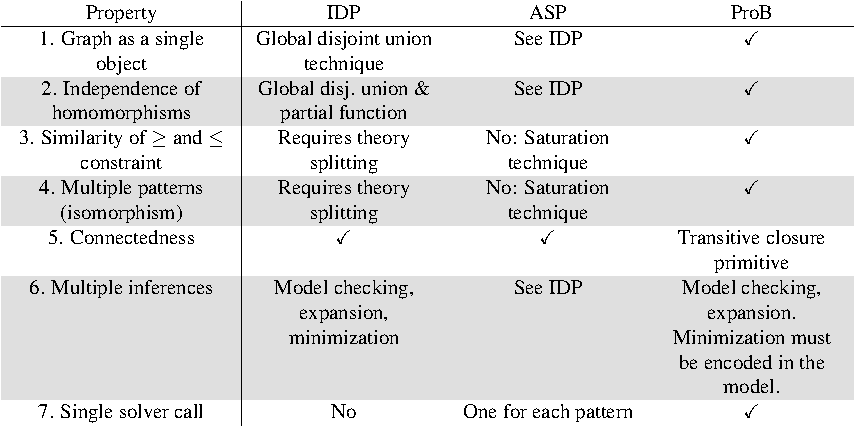
\includegraphics[scale=0.75]{PropertyTable-crop.pdf}
\end{center}
\caption{Evaluation of the desirable properties in IDP / ASP / ProB\label{tbl:conclusion} for modeling the general graph mining problem based on its key components (matching, pattern enumeration, etc)}
\vspace{-3em}
\end{table}
